\section{Introduzione}
\subsection{Scopo del prodotto}
Lo scopo è quello di fornire uno strumento intuitivo e immersivo per gli utenti che voglio partecipare all'esperienza di esplorare un acquario con i suoi ornamenti e decorazioni.
\newline
Le decorazioni vengono così esposte e visualizzate in un modo molto più autentico e coinvolgente.

\subsection{Descrizione generale}
Per rendere il documento il più esauriente possibile ma allo stesso tempo non troppo prolisso, abbiamo schematizzato ogni caso d'uso evidenziando:  precondizioni, postcondizioni, scenario principale in cui tale azione avrà luogo, una breve descrizione ed eventuali estensioni.\newline
In alcuni casi è stata anche inserita un'immagine dello schema UML per fornire una spiegazione visiva che può aiutare nel comprendere più a fondo il nostro lavoro.\newline
Da notare, nelle immagini dello schema UML sono stati rappresentati in azzurro i casi d'uso facoltativi.

\subsection{Attori}
Data l'ampiezza e struttura ridotta del software, l'attore che interagisce col nostro software è uno solo, denominato "Utente in ambiente 3D". 

\subsubsection{Utente in ambiente 3D}
Si tratta dell'utente protagonista di tutti i casi d'uso del nostro prodotto, chiamato tale dato che il software fornisce un immersione completa all'interno dello scenario 3D. \newline
L'utente non verrai mai reindirizzato a una normale pagina web statica, poiché ne risentirebbe la user experience. 

\section{Casi d'uso}

\subsection{UC 1 - Rimozione oggetti dal carrello}

\begin{figure}[H]
  \renewcommand{\thefigure}{1}
  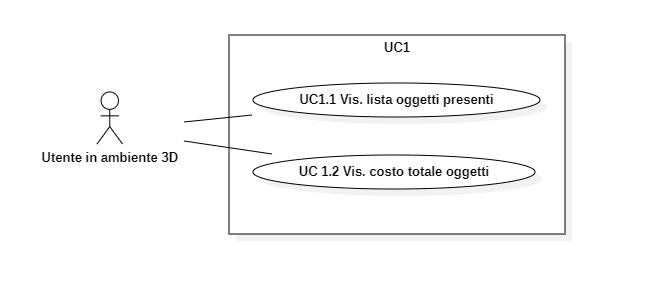
\includegraphics[width=\linewidth]{./res/images/UC1.png}
  \caption{UC 1 - Rimozione oggetti dal carrello}
  \label{fig:UC 1}
\end{figure}

\begin{itemize}
	
	\item Attore primario: 
	\begin{itemize}
		\item Utente in ambiente 3D.
	\end{itemize}
	\item Descrizione:
	\begin{itemize}
		\item Vengono rimossi uno o più oggetti.
	\end{itemize}
	
	\item Precondizioni:
	\begin{itemize}
		\item Il carrello contiene almeno un oggetto.
	\end{itemize}
	
	\item Postcondizioni:
	\begin{itemize}
		\item Uno o più oggetti sono stati rimossi dal carrello;
		\item Il carrello potrebbe essere vuoto.
	\end{itemize}
	
	\item Scenario principale:
	\begin{itemize}
		\item L'utente interagisce con il sistema per effettuare la rimozione di uno o più oggetti dal carrello.
	\end{itemize}
	
\end{itemize}


\subsubsection{UC 1.1 - Rimozione oggetto singolo dal carrello}

\begin{itemize}
	
	\item Attore primario: 
	\begin{itemize}
		\item Utente in ambiente 3D.
	\end{itemize}
	\item Descrizione:
	\begin{itemize}
		\item Viene rimosso un singolo oggetto dal carrello.
	\end{itemize}
	
	\item Precondizioni:
	\begin{itemize}
		\item Il carrello contiene almeno un oggetto.
	\end{itemize}
	
	\item Postcondizioni:
	\begin{itemize}
		\item Un oggetto è stato rimosso dal carrello;
		\item Il carrello potrebbe essere vuoto.
	\end{itemize}
	
	\item Scenario principale:
	\begin{itemize}
		\item L'utente interagisce con il sistema per la rimozione di un oggetto dal carrello.
	\end{itemize}
	
\end{itemize}

\subsubsection{UC 1.2 - Svuotamento totale carrello}
\begin{itemize}
	
	\item Attore primario: 
	\begin{itemize}
		\item Utente in ambiente 3D.
	\end{itemize}
	\item Descrizione:
	\begin{itemize}
		\item Prevede la rimozione di tutti gli oggetti presenti nel carrello con un singolo comando.
	\end{itemize}
	
	\item Precondizioni:
	\begin{itemize}
		\item Il carrello contiene almeno un oggetto.
	\end{itemize}
	
	\item Postcondizioni:
	\begin{itemize}
		\item Tutti gli oggetti sono stati rimossi dal carrello;
		\item Il carrello è vuoto.
	\end{itemize}
	
	\item Scenario principale:
	\begin{itemize}
		\item L'utente interagisce con il sistema per svuotare completamente il carrello.
	\end{itemize}
	
\end{itemize}

\pagebreak

\subsection{UC 2 - Visualizzazione contenuto del carrello}

\begin{figure}[H]
  \renewcommand{\thefigure}{2}
  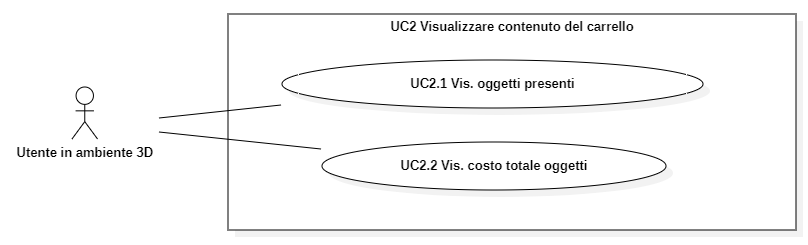
\includegraphics[width=\linewidth]{./res/images/UC2.png}
  \caption{UC 2 - Visualizzazione contenuto del carrello}
  \label{fig:UC 2}
\end{figure}

\begin{itemize}
	
	\item Attore primario: 
	\begin{itemize}
		\item Utente in ambiente 3D.
	\end{itemize}
	\item Descrizione:
	\begin{itemize}
		\item Permette di visualizzare il contenuto del carrello.
	\end{itemize}
	
	\item Precondizioni:
	\begin{itemize}
		\item Il contenuto del carrello è nascosto.
	\end{itemize}
	
	\item Postcondizioni:
	\begin{itemize}
		\item Il contenuto del carrello è visibile.
	\end{itemize}
	
	\item Scenario principale:
	\begin{itemize}
		\item L'utente interagisce con il sistema per visualizzare il contenuto del carrello.
	\end{itemize}
	
\end{itemize}

\subsubsection{UC 2.1 - Visualizzazione oggetti presenti con relative caratteristiche e quantità}

\begin{figure}[H]
  \renewcommand{\thefigure}{3}
  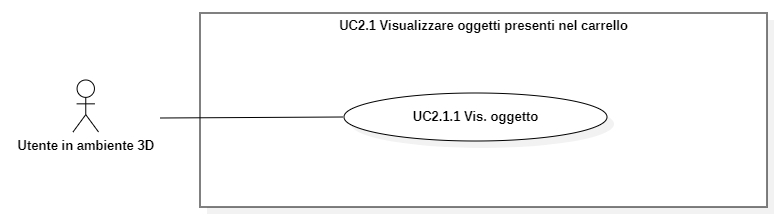
\includegraphics[width=\linewidth]{./res/images/UC2.1.png}
  \caption{UC 2.1 - Visualizzazione oggetti presenti con relative caratteristiche e quantità}
  \label{fig:UC 2.1}
\end{figure}

\begin{itemize}
	
	\item Attore primario: 
	\begin{itemize}
		\item Utente in ambiente 3D.
	\end{itemize}
	\item Descrizione:
	\begin{itemize}
		\item L'utente può visualizzare la lista degli oggetti presenti nel carrello.
	\end{itemize}
	
	\item Precondizioni:
	\begin{itemize}
		\item Il contenuto del carrello è visibile.
	\end{itemize}
	
	\item Postcondizioni:
	\begin{itemize}
		\item Il contenuto del carrello è visibile;
		\item La lista degli oggetti presenti all'interno del carrello è visibile.
	\end{itemize}
	
	\item Scenario principale:
	\begin{itemize}
		\item Nessuna azione richiesta.
	\end{itemize}
	
\end{itemize}

\paragraph{UC 2.1.1 - Visualizzazione oggetto}

\begin{figure}[H]
  \renewcommand{\thefigure}{4}
  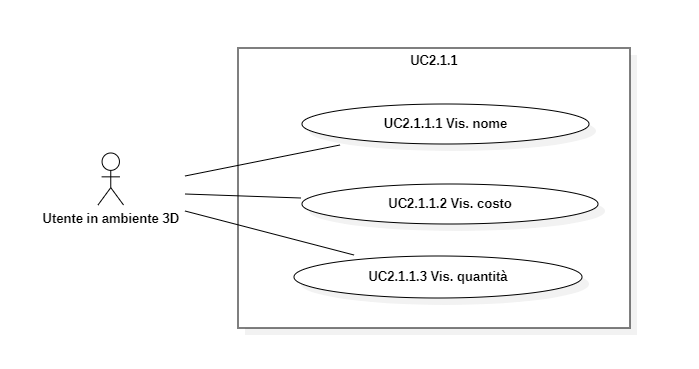
\includegraphics[width=\linewidth]{./res/images/UC2.1.1.png}
  \caption{UC 2.1.1 - Visualizzazione oggetto}
  \label{fig:UC 2.1.1}
\end{figure}

\begin{itemize}
	
	\item Attore primario: 
	\begin{itemize}
		\item Utente in ambiente 3D.
	\end{itemize}
	\item Descrizione:
	\begin{itemize}
		\item Prevede la visualizzazione la visualizzazione di un oggetto all'interno della lista oggetti del carrello.
	\end{itemize}
	
	\item Precondizioni:
	\begin{itemize}
		\item La lista degli oggetti presenti all'interno del carrello è visibile.
	\end{itemize}
	
	\item Postcondizioni:
	\begin{itemize}
		\item La lista degli oggetti presenti all'interno del carrello è visibile;
		\item L'oggetto è visibile nella lista oggetti del carrello.
	\end{itemize}
	
	\item Scenario principale:
	\begin{itemize}
		\item Nessuna azione richiesta.
	\end{itemize}
	
\end{itemize}

\subparagraph{UC 2.1.1.1 - Visualizzazione icona}
\begin{itemize}
	
	\item Attore primario: 
	\begin{itemize}
		\item Utente in ambiente 3D.
	\end{itemize}
	\item Descrizione:
	\begin{itemize}
		\item Prevede la visualizzazione di un'icona associata all'oggetto a cui fa riferimento, l'icona è un'anteprima miniaturizzata dell'oggetto a cui fa riferimento.
	\end{itemize}
	
	\item Precondizioni:
	\begin{itemize}
		\item L'oggetto è visibile nella lista oggetti del carrello.
	\end{itemize}
	
	\item Postcondizioni:
	\begin{itemize}
		\item L'oggetto è visibile nella lista oggetti del carrello;
		\item L'icona associata all'oggetto è visibile.
	\end{itemize}
	
	\item Scenario principale:
	\begin{itemize}
		\item Nessuna azione richiesta.
	\end{itemize}
	
\end{itemize}

\subparagraph{UC 2.1.1.2 - Visualizzazione nome}
\begin{itemize}
	
	\item Attore primario: 
	\begin{itemize}
		\item Utente in ambiente 3D.
	\end{itemize}
	\item Descrizione:
	\begin{itemize}
		\item Prevede la visualizzazione del nome dell'oggetto, il nome dell'oggetto è un identificativo che permette di distinguere oggetti diversi tra loro.
	\end{itemize}
	
	\item Precondizioni:
	\begin{itemize}
		\item L'oggetto è visibile nella lista oggetti del carrello.
	\end{itemize}
	
	\item Postcondizioni:
	\begin{itemize}
		\item L'oggetto è visibile nella lista oggetti del carrello;
		\item Il nome associato all'oggetto è visibile.
	\end{itemize}
	
	\item Scenario principale:
	\begin{itemize}
		\item Nessuna azione richiesta.
	\end{itemize}
	
\end{itemize}

\subparagraph{UC 2.1.1.3 - Visualizzazione costo}
\begin{itemize}
	
	\item Attore primario: 
	\begin{itemize}
		\item Utente in ambiente 3D.
	\end{itemize}
	\item Descrizione:
	\begin{itemize}
		\item Prevede la visualizzazione del costo dell'oggetto.
	\end{itemize}
	
	\item Precondizioni:
	\begin{itemize}
		\item L'oggetto è visibile nella lista oggetti del carrello.
	\end{itemize}
	
	\item Postcondizioni:
	\begin{itemize}
		\item L'oggetto è visibile nella lista oggetti del carrello;
		\item Il costo associato all'oggetto è visibile.
	\end{itemize}
	
	\item Scenario principale:
	\begin{itemize}
		\item Nessuna azione richiesta.
	\end{itemize}
	
\end{itemize}

\subparagraph{UC 2.1.1.4 - Visualizzazione quantità}
\begin{itemize}
	
	\item Attore primario: 
	\begin{itemize}
		\item Utente in ambiente 3D.
	\end{itemize}
	\item Descrizione:
	\begin{itemize}
		\item Prevede la visualizzazione del numero di oggetti identici all'oggetto (compreso) presenti all'interno del carrello.
	\end{itemize}
	
	\item Precondizioni:
	\begin{itemize}
		\item L'oggetto è visibile nella lista oggetti del carrello.
	\end{itemize}
	
	\item Postcondizioni:
	\begin{itemize}
		\item L'oggetto è visibile nella lista oggetti del carrello;
		\item La quantità di oggetti identici all'oggetto (compreso) è visibile.
	\end{itemize}
	
	\item Scenario principale:
	\begin{itemize}
		\item Nessuna azione richiesta.
	\end{itemize}
	
\end{itemize}

\subparagraph{UC 2.1.1.5 - Visualizzazione caratteristiche fisiche}
\begin{itemize}
	
	\item Attore primario: 
	\begin{itemize}
		\item Utente in ambiente 3D.
	\end{itemize}
	\item Descrizione:
	\begin{itemize}
		\item Prevede la visualizzazione delle caratteristiche fisiche dell'oggetto.
	\end{itemize}
	
	\item Precondizioni:
	\begin{itemize}
		\item L'oggetto è visibile nella lista oggetti del carrello.
	\end{itemize}
	
	\item Postcondizioni:
	\begin{itemize}
		\item L'oggetto è visibile nella lista oggetti del carrello;
		\item Le caratteristiche fisiche dell'oggetto sono visibili.
	\end{itemize}
	
	\item Scenario principale:
	\begin{itemize}
		\item Nessuna azione richiesta.
	\end{itemize}
	
\end{itemize}

\subsubsection{UC 2.2 - Visualizzazione costo totale oggetti}
\begin{itemize}
	
	\item Attore primario: 
	\begin{itemize}
		\item Utente in ambiente 3D.
	\end{itemize}
	\item Descrizione:
	\begin{itemize}
		\item Prevede la visualizzazione della somma di tutti i costi degli oggetti presenti all'interno del carrello.
	\end{itemize}
	
	\item Precondizioni:
	\begin{itemize}
		\item Il contenuto del carrello è visibile.
	\end{itemize}
	
	\item Postcondizioni:
	\begin{itemize}
		\item Il contenuto del carrello è visibile;
		\item Il totale della somma di tutti i costi degli oggetti presenti nel carrello è visibile.
	\end{itemize}
	
	\item Scenario principale:
	\begin{itemize}
		\item Nessuna azione richiesta.
	\end{itemize}
	
\end{itemize}

\pagebreak

\subsection{UC 3 - Aggiungere un oggetto al carrello}
\begin{itemize}

	\item Attore primario: 
	\begin{itemize}
		\item Utente in ambiente 3D.
	\end{itemize}
	\item Descrizione:
	\begin{itemize}
		\item Aggiungere un oggetto al carrello significa aggiungere alla lista degli oggetti presenti nel carrello l'oggetto desiderato e visualizzare un messaggio di oggetto aggiunto al carrello con successo.
\newline L'oggetto all'interno dell'ambiente continua ad esistere anche dopo la sua aggiunta al carrello.
	\end{itemize}
	
	\item Precondizioni:
	\begin{itemize}
		\item L'oggetto da aggiungere al carrello si trova all'interno dell'ambiente 3D.
	\end{itemize}
	
	\item Postcondizioni:
	\begin{itemize}
		\item L'oggetto aggiunto al carrello si trova all'interno dell'ambiente 3D;
		\item L'oggetto e' presente all'interno del carrello.
	\end{itemize}
	
	\item Scenario principale:
	\begin{itemize}
		\item L'utente interagisce con l'oggetto da aggiungere all'interno del carrello;
		\item L'utente seleziona il comando aggiungi oggetto al carrello.
	\end{itemize}
	
\end{itemize}

\pagebreak

\subsection{UC 4 - Compiere azioni di movimento}

\begin{figure}[H]
  \renewcommand{\thefigure}{5}
  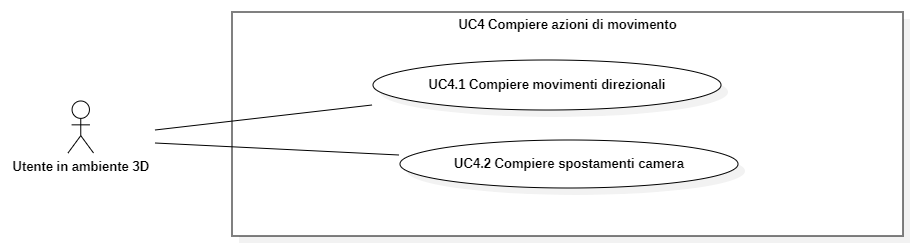
\includegraphics[width=\linewidth]{./res/images/UC4.png}
  \caption{UC 4 - Compiere azioni di movimento}
  \label{fig:UC 4}
\end{figure}

\begin{itemize}

	\item Attore primario: 
	\begin{itemize}
		\item Utente in ambiente 3D.
	\end{itemize}
	\item Descrizione:
	\begin{itemize}
		\item Compiere azioni di movimento significa interagire con il sistema per esplorare l'ambiente 3D.
\newline La posizione dell'utente all'interno dell'ambiente 3D comprende sia la sua posizione nello spazio che l'orientamento
della sua visuale.
	\end{itemize}
	
	\item Precondizioni:
	\begin{itemize}
		\item Le azioni di movimento richieste dall'utente devono essere abilitate;
		\item Le azioni di movimento richieste dall'utente devono essere valide;
		\item L'utente si trova in una posizione iniziale.
	\end{itemize}
	
	\item Postcondizioni:
	\begin{itemize}
		\item L'utente si trova in una posizione diversa da quella iniziale.
	\end{itemize}
	
	\item Scenario principale:
	\begin{itemize}
		\item L'utente interagisce con il sistema per compiere un'azione di movimento.
	\end{itemize}
	
\end{itemize}

\subsubsection{UC 4.1 - Compiere movimenti direzionali}

\begin{figure}[H]
  \renewcommand{\thefigure}{6}
  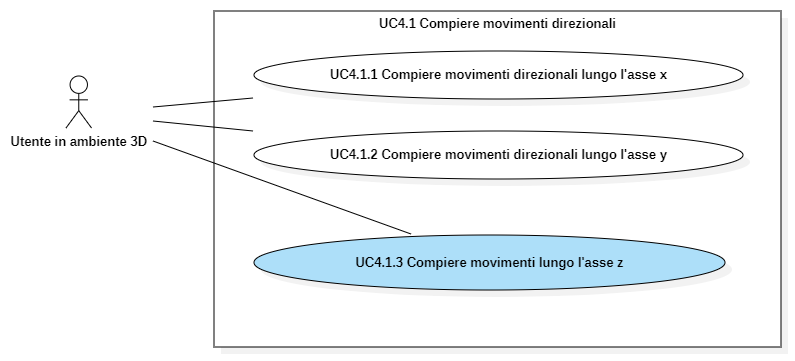
\includegraphics[width=\linewidth]{./res/images/UC4.1.png}
  \caption{UC 4.1 - Compiere movimenti direzionali}
  \label{fig:UC 4.1}
\end{figure}

\begin{itemize}

	\item Attore primario: 
	\begin{itemize}
		\item Utente in ambiente 3D.
	\end{itemize}
	\item Descrizione:
	\begin{itemize}
		\item Compiere azioni di movimenti direzionali significa interagire con il sistema per spostarsi nello spazio offerto dall'ambiente 3D.
\newline Attenzione: anche se dei movimenti direzionali non fossero offerti all'utente non e' detto che non si possa spostare in quella direzione,infatti,alcuni spostamenti direzionali potrebbero dipendere da vincoli imposti dall'ambiente 3D (esempio la presenza di un dislivello o la presenza di scale ecc...).
	\end{itemize}
	
	\item Precondizioni:
	\begin{itemize}
		\item Le azioni di movimento direzionali devono essere abilitate;
		\item Le azioni di movimento direzionali devono essere valide;
		\item L'utente si trova in una posizione iniziale nello spazio.
	\end{itemize}
	
	\item Postcondizioni:
	\begin{itemize}
		\item L'utente si trova in una posizione diversa da quella iniziale nello spazio.
	\end{itemize}
	
	\item Scenario principale:
	\begin{itemize}
		\item L'utente interagisce con il sistema per compiere un'azione di movimento direzionale.
	\end{itemize}
	
\end{itemize}

\paragraph{UC 4.1.1 - Compiere movimenti direzionali lungo l'asse X}
\begin{itemize}

	\item Attore primario: 
	\begin{itemize}
		\item Utente in ambiente 3D.
	\end{itemize}
	\item Descrizione:
	\begin{itemize}
		\item Caso d'uso autoesplicativo.
	\end{itemize}
	
	\item Precondizioni:
	\begin{itemize}
		\item Le azioni di movimento direzionale lungo l'asse delle X devono essere abilitate;
		\item Le azioni di movimento direzionali lungo l'asse X devono essere valide;
		\item L'utente si trova in una posizione iniziale nello spazio rispetto all'asse X.
	\end{itemize}
	
	\item Postcondizioni:
	\begin{itemize}
		\item L'utente si trova in una posizione diversa da quella iniziale nello spazio rispetto all'asse X.
	\end{itemize}
	
	\item Scenario principale:
	\begin{itemize}
		\item L'utente interagisce con il sistema per compiere un'azione di movimento direzionale lungo l'asse X.
	\end{itemize}
	
\end{itemize}

\paragraph{UC 4.1.2 - Compiere movimenti direzionali lungo l'asse Y}
\begin{itemize}

	\item Attore primario: 
	\begin{itemize}
		\item Utente in ambiente 3D.
	\end{itemize}
	\item Descrizione:
	\begin{itemize}
		\item Caso d'uso autoesplicativo.
	\end{itemize}
	
	\item Precondizioni:
	\begin{itemize}
		\item Le azioni di movimento direzionale lungo l'asse delle Y devono essere abilitate;
		\item Le azioni di movimento direzionali lungo l'asse Y devono essere valide;
		\item L'utente si trova in una posizione iniziale nello spazio rispetto all'asse Y.
	\end{itemize}
	
	\item Postcondizioni:
	\begin{itemize}
		\item L'utente si trova in una posizione diversa da quella iniziale nello spazio rispetto all'asse Y.
	\end{itemize}
	
	\item Scenario principale:
	\begin{itemize}
		\item L'utente interagisce con il sistema per compiere un'azione di movimento direzionale lungo l'asse Y.
	\end{itemize}
	
\end{itemize}

\paragraph{UC 4.1.3 - Compiere movimenti direzionali lungo l'asse Z}
\begin{itemize}

	\item Attore primario: 
	\begin{itemize}
		\item Utente in ambiente 3D.
	\end{itemize}
	\item Descrizione:
	\begin{itemize}
		\item Caso d'uso autoesplicativo.
	\end{itemize}
	
	\item Precondizioni:
	\begin{itemize}
		\item Le azioni di movimento direzionale lungo l'asse delle Z devono essere abilitate;
		\item Le azioni di movimento direzionali lungo l'asse Z devono essere valide;
		\item L'utente si trova in una posizione iniziale nello spazio rispetto all'asse Z.
	\end{itemize}
	
	\item Postcondizioni:
	\begin{itemize}
		\item L'utente si trova in una posizione diversa da quella iniziale nello spazio rispetto all'asse Z.
	\end{itemize}
	
	\item Scenario principale:
	\begin{itemize}
		\item L'utente interagisce con il sistema per compiere un'azione di movimento direzionale lungo l'asse Z.
	\end{itemize}
	
\end{itemize}

\subsubsection{UC 4.2 - Compiere rotazioni camera}
\begin{itemize}

	\item Attore primario: 
	\begin{itemize}
		\item Utente in ambiente 3D.
	\end{itemize}
	\item Descrizione:
	\begin{itemize}
		\item Compiere un'azione di rotazione camera permette all'utente di vedere l'ambiente che lo circonda variando
la direzione della propria visuale.
\newline Non ci sono vincoli alle direzioni in cui può variare lo spostamento della camera.
	\end{itemize}
	
	\item Precondizioni:
	\begin{itemize}
		\item L'azione di spostamento camera deve essere abilitata;
		\item La visuale dell'utente è direzionata verso un punto iniziale.
	\end{itemize}
	
	\item Postcondizioni:
	\begin{itemize}
		\item La visuale dell'utente è direzionata verso un punto diverso rispetto a quello iniziale.
	\end{itemize}
	
	\item Scenario principale:
	\begin{itemize}
		\item L'utente interagisce con il sistema per compiere un'azione di spostamento camera.
	\end{itemize}
	
\end{itemize}

\pagebreak

\subsection{UC 5 - Modificare attributi oggetto}
\begin{itemize}

	\item Attore primario: 
	\begin{itemize}
		\item Utente in ambiente 3D.
	\end{itemize}
	\item Descrizione:
	\begin{itemize}
		\item Modificare attributi oggetto prevede la modifica degli attributi dell'oggetto che l'utente desidera modificare.
\newline A seconda dell'oggetto da modificare gli attributi modificabili potrebbero essere diversi.
\newline Potrebbero essere presenti anche oggetti non modificabili.
	\end{itemize}
	
	\item Precondizioni:
	\begin{itemize}
		\item L'oggetto da modificare si trova all'interno dell'ambiente 3D.
	\end{itemize}
	
	\item Postcondizioni:
	\begin{itemize}
		\item L'oggetto modificato si trova all'interno dell'ambiente 3D;
		\item L'oggetto è stato modificato;
		\item L'oggetto assume le caratteristiche visive dovute alle. modifiche
	\end{itemize}
	
	\item Scenario principale:
	\begin{itemize}
		\item L'utente interagisce con l'oggetto da modificare;
		\item L'utente seleziona il comando modifica oggetto;
		\item L'utente apporta le modifiche desiderate;
		\item L'utente conferma le modifiche.
	\end{itemize}
	
	\item Estensioni:
	\begin{itemize}
		\item UC 6 - Visualizzazione messaggio oggetto non modificabile.
	\end{itemize}
	
\end{itemize}

\pagebreak

\subsection{UC 6 - Visualizzazione messaggio oggetto non modificabile}
\begin{itemize}

	\item Attore primario: 
	\begin{itemize}
		\item Utente in ambiente 3D.
	\end{itemize}
	\item Descrizione:
	\begin{itemize}
		\item Prevede la visualizzazione di un messaggio informativo di "oggetto non modificabile".
\newline Un oggetto potrebbe non essere modificabile per la presenza di una sola configurazione per quell'oggetto.
	\end{itemize}
	
	\item Precondizioni:
	\begin{itemize}
		\item L'oggetto da modificare si trova all'interno dell'ambiente 3D;
		\item L'oggetto desiderato non è modificabile.
	\end{itemize}
	
	\item Postcondizioni:
	\begin{itemize}
		\item L'oggetto non è stato modificato;
		\item L'oggetto mantiene le sue caratteristiche visive.
	\end{itemize}
	
	\item Scenario principale:
	\begin{itemize}
		\item L'utente interagisce con l'oggetto da modificare;
		\item L'utente seleziona il comando modifica oggetto.
	\end{itemize}
	
\end{itemize}

\pagebreak

\subsection{UC 7 - Visualizzazione contenuto lista oggetti}

\begin{figure}[H]
  \renewcommand{\thefigure}{7}
  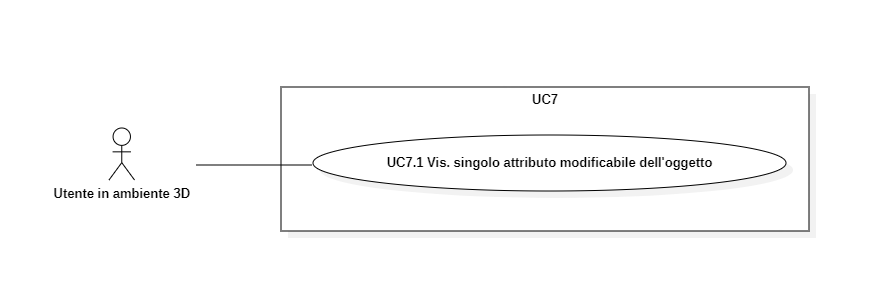
\includegraphics[width=\linewidth]{./res/images/UC7.png}
  \caption{UC 7 - Visualizzazione contenuto lista oggetti}
  \label{fig:UC 7}
\end{figure}

\begin{itemize}

	\item Attore primario: 
	\begin{itemize}
		\item Utente in ambiente 3D.
	\end{itemize}
	\item Descrizione:
	\begin{itemize}
		\item Visualizza contenuto lista oggetti permette di visualizzare il contenuto della lista oggetti.
	\end{itemize}
	
	\item Precondizioni:
	\begin{itemize}
		\item Il contenuto della lista oggetti è nascosto.
	\end{itemize}
	
	\item Postcondizioni:
	\begin{itemize}
		\item Il contenuto della lista oggetti è visibile.
	\end{itemize}
	
	\item Scenario principale:
	\begin{itemize}
		\item L'utente interagisce con il sistema per rendere il contenuto della lista oggetti visibile.
	\end{itemize}
	
\end{itemize}

\subsubsection{UC 7.1 - Visualizzazione oggetti stanza attuale}
\begin{itemize}

	\item Attore primario: 
	\begin{itemize}
		\item Utente in ambiente 3D.
	\end{itemize}
	\item Descrizione:
	\begin{itemize}
		\item Visualizza oggetti stanza attuale prevede la visualizzazione di una lista di oggetti contenente gli oggetti della stanza in
cui l'utente si trova.
	\end{itemize}
	
	\item Precondizioni:
	\begin{itemize}
		\item Il contenuto della lista oggetti è visibile.
	\end{itemize}
	
	\item Postcondizioni:
	\begin{itemize}
		\item Gli oggetti contenuti nella lista oggetti sono visibili.
	\end{itemize}
	
	\item Scenario principale:
	\begin{itemize}
		\item Nessuna azione richiesta.
	\end{itemize}
	
\end{itemize}

\pagebreak

\subsection{UC 8 - Visualizzazione dettagli oggetto}
\begin{itemize}

	\item Attore primario: 
	\begin{itemize}
		\item Utente in ambiente 3D.
	\end{itemize}
	\item Descrizione:
	\begin{itemize}
		\item Visualizza dettagli oggetto prevede la visualizzazione dei dettagli di un oggetto.
	\end{itemize}
	
	\item Precondizioni:
	\begin{itemize}
		\item I dettagli dell'oggetto non sono visibili.
	\end{itemize}
	
	\item Postcondizioni:
	\begin{itemize}
		\item I dettagli dell'oggetto sono visibili.
	\end{itemize}
	
	\item Scenario principale:
	\begin{itemize}
		\item L'utente interagisce con il sistema per rendere visibili i dettagli di un oggetto.
	\end{itemize}
	
\end{itemize}

\pagebreak

\subsection{UC 9 - Riposizionamento}

\begin{figure}[H]
  \renewcommand{\thefigure}{8}
  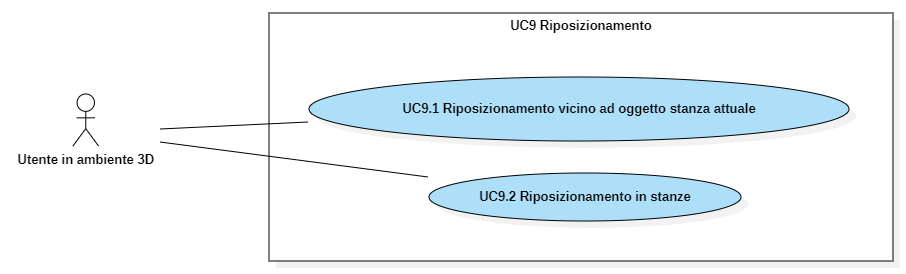
\includegraphics[width=\linewidth]{./res/images/UC9.png}
  \caption{UC 9 - Riposizionamento}
  \label{fig:UC 9}
\end{figure}

\begin{itemize}

	\item Attore primario: 
	\begin{itemize}
		\item Utente in ambiente 3D.
	\end{itemize}
	\item Descrizione:
	\begin{itemize}
		\item Riposizionamento permette all'utente di posizionarsi in punti prestabiliti all'interno dell'ambiente 3D.
	\end{itemize}
	
	\item Precondizioni:
	\begin{itemize}
		\item L'utente si trova in un punto di partenza.
	\end{itemize}
	
	\item Postcondizioni:
	\begin{itemize}
		\item L'utente si trova in un punto diverso da quello di partenza prestabilito dal sistema.
	\end{itemize}
	
	\item Scenario principale:
	\begin{itemize}
		\item L'utente interagisce con il sistema per riposizionarsi in un punto diverso all'interno dell'ambiente 3D.
	\end{itemize}
	
\end{itemize}

\subsubsection{UC 9.1 - Riposizionamento vicino ad oggetto stanza attuale}
\begin{itemize}

	\item Attore primario: 
	\begin{itemize}
		\item Utente in ambiente 3D.
	\end{itemize}
	\item Descrizione:
	\begin{itemize}
		\item Riposizionamento vicino ad oggetto stanza attuale prevede il riposizionamento dell'utente vicino ad un oggetto
della stanza in cui si trova.
	\end{itemize}
	
	\item Precondizioni:
	\begin{itemize}
		\item L'utente si trova in un punto di partenza.
	\end{itemize}
	
	\item Postcondizioni:
	\begin{itemize}
		\item L'utente si trova nelle vicinanze dell'oggetto desiderato in un punto prestabilito.
	\end{itemize}
	
	\item Scenario principale:
	\begin{itemize}
		\item L'utente seleziona il comando per riposizionarsi nelle vicinanze di un oggetto.
	\end{itemize}
	
\end{itemize}

\subsubsection{UC 9.2 - Riposizionamento in stanze}
\begin{itemize}

	\item Attore primario: 
	\begin{itemize}
		\item Utente in ambiente 3D.
	\end{itemize}
	\item Descrizione:
	\begin{itemize}
		\item Riposizionamento in stanze prevede il riposizionamento dell'utente in un punto prestabilito di una stanza da lui selezionata.
	\end{itemize}
	
	\item Precondizioni:
	\begin{itemize}
		\item L'utente si trova in un punto di partenza di una determinata stanza.
	\end{itemize}
	
	\item Postcondizioni:
	\begin{itemize}
		\item L'utente si trova in un punto prestabilito di una stanza da lui selezionata.
	\end{itemize}
	
	\item Scenario principale:
	\begin{itemize}
		\item L'utente seleziona il comando per riposizionarsi nella stanza. desiderata
	\end{itemize}
	
\end{itemize}

\pagebreak

\subsection{UC 10 - Riposizionamento non concesso}
\begin{itemize}

	\item Attore primario: 
	\begin{itemize}
		\item Utente in ambiente 3D.
	\end{itemize}
	\item Descrizione:
	\begin{itemize}
		\item Se l'utente si trova in prossimità del punto di destinazione, il riposizionamento non avviene.
	\end{itemize}
	
	\item Precondizioni:
	\begin{itemize}
		\item L'utente si trova in prossimità del punto di destinazione;
		\item L'utente interagisce con il comando di riposizionamento in quella destinazione.
	\end{itemize}
	
	\item Postcondizioni:
	\begin{itemize}
		\item L'utente si trova in prossimità del punto di destinazione;
		\item Il riposizionamento non è stato effettuato.
	\end{itemize}
	
	\item Scenario principale:
	\begin{itemize}
		\item Nessuna azione richiesta.
	\end{itemize}
	
\end{itemize}

\pagebreak

\subsection{UC 11 - Visualizzazione contenuto lista stanze}
\begin{itemize}

	\item Attore primario: 
	\begin{itemize}
		\item Utente in ambiente 3D.
	\end{itemize}
	\item Descrizione:
	\begin{itemize}
		\item Visualizzazione contenuto lista stanze permette di visualizzare il contenuto della lista stanze.
\newline Il contenuto della lista stanze prevede l'elenco delle stanze presenti all'interno dell'ambiente 3D.
	\end{itemize}
	
	\item Precondizioni:
	\begin{itemize}
		\item Il contenuto della lista stanze è nascosto.
	\end{itemize}
	
	\item Postcondizioni:
	\begin{itemize}
		\item Il contenuto della lista stanze è visibile.
	\end{itemize}
	
	\item Scenario principale:
	\begin{itemize}
		\item L'utente interagisce con il sistema per rendere il contenuto della lista stanze visibile.
	\end{itemize}
	
\end{itemize}

\pagebreak

\subsection{UC 12 - Spostamento oggetto}
\begin{itemize}

	\item Attore primario: 
	\begin{itemize}
		\item Utente in ambiente 3D.
	\end{itemize}
	\item Descrizione:
	\begin{itemize}
		\item Riposizionamento di un oggetto in un altro punto della stanza in cui ci si trova.
	\end{itemize}
	
	\item Precondizioni:
	\begin{itemize}
		\item L'oggetto da spostare si trova all'interno dell'ambiente 3D;
		\item L'oggetto si trova in una coordinata X, Y, Z di una stanza.
	\end{itemize}
	
	\item Postcondizioni:
	\begin{itemize}
		\item L'oggetto si trova in una coordinata X, Y, Z diversa da quella di partenza nella stessa stanza.
	\end{itemize}
	
	\item Scenario principale:
	\begin{itemize}
		\item L'utente interagisce con l'oggetto per poterlo spostare in un altra coordinata all'interno della stanza di partenza.
	\end{itemize}
	
	\item Estensioni:
	\begin{itemize}
		\item UC 13 - Oggetto non posizionato.
	\end{itemize}
	
\end{itemize}

\pagebreak

\subsection{UC 13 - Oggetto non posizionato}
\begin{itemize}

	\item Attore primario: 
	\begin{itemize}
		\item Utente in ambiente 3D.
	\end{itemize}
	\item Descrizione:
	\begin{itemize}
		\item Se l'utente cerca di posizionare un oggetto in una coordinata X, Y, Z non legittima, l'oggetto non viene posizionato.
	\end{itemize}
	
	\item Precondizioni:
	\begin{itemize}
		\item L'oggetto si trova in una coordinata X, Y, Z non valida;
		\item L'oggetto è in fase di spostamento.
	\end{itemize}
	
	\item Postcondizioni:
	\begin{itemize}
		\item L'oggetto è in fase di spostamento;
		\item L'oggetto non è stato posizionato.
	\end{itemize}
	
	\item Scenario principale:
	\begin{itemize}
		\item Nessuna azione richiesta.
	\end{itemize}
	
\end{itemize}

\pagebreak

\subsection{UC 14 - Torcia}
\begin{itemize}

	\item Attore primario: 
	\begin{itemize}
		\item Utente in ambiente 3D.
	\end{itemize}
	\item Descrizione:
	\begin{itemize}
		\item L'utente può utilizzare una torcia per illuminare parte dell'ambiente di fronte a lui. \newline La torcia si può trovare in due stati, accesa o spenta.
	\end{itemize}
	
	\item Precondizioni:
	\begin{itemize}
		\item La torcia si trova in uno stato iniziale.
	\end{itemize}
	
	\item Postcondizioni:
	\begin{itemize}
		\item La torcia si trova in uno stato finale.
	\end{itemize}
	
	\item Scenario principale:
	\begin{itemize}
		\item L'utente cambia lo stato della torcia.
	\end{itemize}
	
\end{itemize}

\pagebreak

\section{Requisiti}

\subsection{Introduzione}
Sono stati definiti dei requisiti codificati in base all'ambito di competenza e ad un numero seriale per tenerne meglio traccia, inoltre nelle tabelle sottostanti sono fornite descrizione e classificazione di ciascun requisito.
\tabularnewline
Il codice di ciascuno requisito è formato da:
\begin{itemize}
	\item R: sta per requisito e serve a definire il dominio del codice rendendo subito intuibile che si tratti di un requisito
	\item Lettera di tipologia:
	\begin{itemize}
		\item F: funzionale
		\item Q: qualitativo
		\item D: di dominio
		\item P: prestazionale
	\end{itemize}
	\item Numero seriale
\end{itemize}

\subsection{Requisiti funzionali}
\reqTable{
	\textbf{RF1} & L'utente deve poter rimuovere uno o più oggetti dal carrello & Facoltativo & UC1 \tabularnewline
	\textbf{RF1.1} & L'utente deve poter rimuovere un oggetto dal carrello & Facoltativo & UC1.1 \tabularnewline
     \textbf{RF1.2} & L'utente deve poter rimuovere tutti gli oggetti dal carrello & Facoltativo & UC1.2\tabularnewline
     
     \textbf{RF2} & L'utente deve poter visualizzare il contenuto del carrello & Obbligatorio & UC2\tabularnewline
     \textbf{RF2.1} & L'utente può visualizzare la lista degli oggetti presenti nel carrello & Obbligatorio & UC2.1\tabularnewline
     \textbf{RF2.2} & L'utente deve poter visualizzare il costo totale degli oggetti presenti nel carrello & Obbligatorio & UC2.2\tabularnewline
     
     \textbf{RF3} & L'utente deve poter aggiungere un oggetto al carrello & Obbligatorio & UC3\tabularnewline
     
     \textbf{RF4} & L'utente deve poter compiere azioni di movimento & Obbligatorio & UC4\tabularnewline
     \textbf{RF4.1} & L'utente deve poter compiere movimenti direzionali & Obbligatorio & UC4.1\tabularnewline
     \textbf{RF4.1.1} & L'utente deve poter compiere movimenti direzionali sull'asse X & Obbligatorio & UC4.1.1\tabularnewline
     \textbf{RF4.1.2} & L'utente deve poter compiere movimenti direzionali sull'asse Y & Obbligatorio & UC4.1.2\tabularnewline
     \textbf{RF4.1.3} & L'utente deve poter compiere movimenti direzionali sull'asse Z & Facoltativo & UC4.1.3\tabularnewline
     \textbf{RF4.2} & L'utente deve poter compiere spostamenti di camera & Obbligatorio & UC4.2\tabularnewline
     
     \textbf{RF15} & L'utente deve poter modificare gli attributi di un oggetto & Obbligatorio & UC5\tabularnewline
     
     \textbf{RF6} & L'utente deve essere notificato in caso un oggetto non fosse modificabile & Obbligatorio & UC6\tabularnewline
     
     \textbf{RF7} & L'utente deve poter visualizzare il contenuto della lista oggetti & Facoltativo & UC7\tabularnewline
     \textbf{RF7.1} & L'utente deve poter visualizzare il contenuto della lista oggetti della stanza attuale & Facoltativo & UC7.1\tabularnewline
     
     \textbf{RF8} & L'utente deve poter visualizzare i dettagli di un oggetto & Obbligatorio & UC8\tabularnewline
     
     \textbf{RF9} & L'utente deve poter riposizionarsi in una coordinata X, Y, Z & Facoltativo & UC9\tabularnewline
     \textbf{RF9.1} & L'utente deve poter riposizionarsi vicino ad un oggetto presente nella stanza & Facoltativo & UC9.1\tabularnewline
     \textbf{RF9.2} & L'utente deve poter riposizionarsi in un punto
prestabilito di una stanza da lui selezionata & Facoltativo & UC9.2\tabularnewline

	\textbf{RF10} & L'utente deve essere notificato quando il riposizionamento non è concesso & Facoltativo & UC10\tabularnewline
	
	\textbf{RF11} & L'utente deve poter visualizzare il contenuto della lista stanze & Facoltativo & UC11\tabularnewline
	
	\textbf{RF12} & L'utente deve poter riposizionare un oggetto presente nella stanza attuale & Facoltativo & UC12\tabularnewline
	
	\textbf{RF13} & L'utente deve non poter riposizionare un oggetto in una coordinata non legittima & Facoltativo & UC13\tabularnewline
	
	\textbf{RF14} & L'utente deve poter utilizzare una torcia per illuminare l'ambiente circostante & Facoltativo & UC14
\\}

\subsection{Requisiti qualitativi}
\reqTable{
	\textbf{RQ1} & Il software deve essere sviluppato seguendo le metriche e il modello di qualità descritti nel documento "Norme di Progetto" & Obbligatorio & Decisione interna \tabularnewline
	\textbf{RQ2} & Il software deve essere sviluppato pubblicando il codice sorgente sul repository Github\textsubscript{g} dedicato & Obbligatorio & Decisione interna \tabularnewline
	\textbf{RQ3} & Il software deve essere sviluppato fornendo una documentazione dettagliata delle varie funzionalità & Obbligatorio & Capitolato
	\\}

\subsection{Requisiti di dominio}
\reqTable{
	\textbf{RD1} & Il software deve essere compatibile con la versione più recente del browser Chrome & Obbligatorio & Decisione interna \tabularnewline
	\textbf{RD2} & Il software deve essere compatibile con la versione più recente del browser Firefox & Obbligatorio & Decisione interna \tabularnewline
	\textbf{RD3} & Il software deve essere compatibile con la versione più recente del browser Safari & Obbligatorio & Decisione interna \tabularnewline
	\textbf{RD4} & Il software deve essere sviluppato utilizzando la libreria Three.js & Obbligatorio & Decisione interna
	\\}

\subsection{Requisiti prestazionali}
\reqTable{
	\textbf{RP1} & Il software deve essere in grado di essere eseguito senza rallentamenti garantendo un esperienza immersiva & Obbligatorio & Decisione interna
	\\}